\section{Monodisperse systems: coexistence pressures}\label{sec:disorderpress}
\begin{figure}
	\begin{center}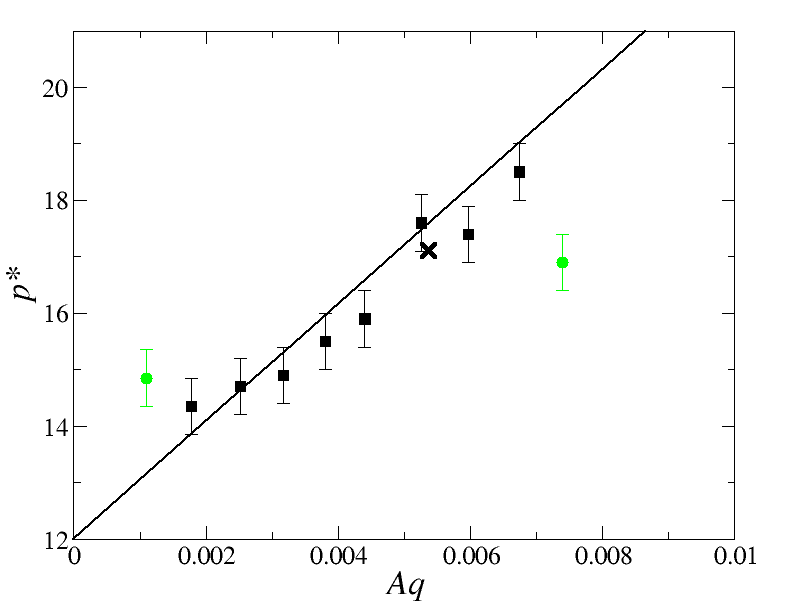
\includegraphics[width=0.8\textwidth]{polydisperse/mono2.png}\end{center}
	\caption[Coexistence pressure vs. $Aq$ for monodisperse systems of aspherical particles]{Coexistence pressure vs. $Aq$ for monodisperse systems of hard aspherical particles with $N_b = 6$, $\sigma_0 = 0.2$.  The line is a fit obtained from the data presented in Figure~\ref{poly} for polydisperse systems with $N_b = 6$, $8$, and $12$.  The cross indicates the position of the polydisperse system with $N_b = 6$, $\sigma_0 = 0.2$.
Points at the extremes of the $q$ distribution are shaded with a lighter color.}\label{mono2}
\end{figure}

The existence of a master curve for the coexistence pressure of significantly different particle distributions (provided $N_b\geq6$), both in terms of their average value  and their width, is quite remarkable, and provides a very compact and elegant way of expressing the equilibrium properties of such systems.  
As a test of the robustness of this relationship, ten monodisperse systems were generated by a single set of parameters: $N_b = 6$, $\sigma_0 = 0.2$.
Each of these systems is characterized, by definition, by an infinitely sharp $P(q)$, and individual configurations were selected to cover a fairly wide range of $Aq$ values, while keeping $A$ roughly constant (because the distribution of $A$ values for a given set $(N_b,\sigma_0)$ is narrow, see Figure~\ref{Ahist}). 
A plot of these data, shown in Figure~\ref{mono2}, indicates that the relationship adapted unaltered from the polydisperse case is a reasonably good predictor of coexistence pressure for the monodisperse case as well.
This is a clear indication that, up to some maximum, the master curve is overall independent of distribution width.

Notice that no coexistence pressures above $p^*(A,q) \simeq 21$ are reported. 
This is not a coincidence; in general, if a system was going to crystallize at all (that is, if the crystalline region of the simulation box was going to grow), the coexistence pressure $p^*$ was below this value.
This is interesting because this value is close to the fluid pressure of a system of hard spheres
at the glass transition density~\cite{speedy}, $p_G = 22.6$, and  it is reasonable to assume that $p_G$ sets an upper bound to the 
largest accessible fluid coexistence pressure for aspherical particles obtained with direct fluid/solid sampling.

In fact, this method  
is clearly susceptible to anomalies in system kinetics, thus making coexistence measurements at pressures larger than the ones herein reported 
quite cumbersome and somewhat unreliable. Nevertheless, if we assume that no aspherical hard particle will easily crystallize above $p_G$, we can 
formulate a prediction for whether a system of aspherical particles should be expected to easily crystallize: given $p^* \simeq 991 Aq + 12$, and based upon this simple line of reasoning, one should expect, as a first-order approximation, a limit of
\begin{equation}Aq \lesssim 0.011 \,.\label{xtallimit}\end{equation}
When the product $Aq$ is below this limit, the system would be expected to easily crystallize at some pressure; above the limit, the system is never expected to crystallize.

\section{Monodisperse systems: predicting crystallization}\label{sec:disorderyesno}

In order to test the prediction above, a large number of monodisperse systems was tested for the simple binary question: ``Does this system crystallize easily?''
In order to answer this question, traditional Monte Carlo simulations were performed in the $NPT$ ensemble.
Instead of intializing the system to be half crystalline and half fluid, a cubic box was used and the simulations was initialized in a fluid state.
Each simulation contained $N = 128$ particles and contained a monodisperse system of aspherical particles constructed with some value of $(N_b, \sigma_0)$; for the purposes of this study, we used $N_b \in \left\{4,6,8,12\right\}$ and $\sigma_0 \in \left(0,1\right)$.

The initial pressure was set to $p = 10$ and the pressure was incremented by $\Delta p = 0.5$ or smaller.
Each simulation was run for a minimum of $4 \cdot 10^6$ Monte Carlo sweeps after thermalization.
The simulation was ended when the system either crystallized or reached a volume fraction $\phi \simeq 0.6$, above the glass transition point of hard sphere, $\phi_G = 0.58$.
Crystallization was detected by a combination of (a) the $q_6$ order parameter, (b) a careful monitoring of the system volume fraction over time for sudden jumps (indicating a phase transition), and (c) visual inspection.
We investigated a total of $487$ different particle geometries. 

Figure~\ref{mono1} summarizes the result of this study. 
\begin{figure}
	\begin{center}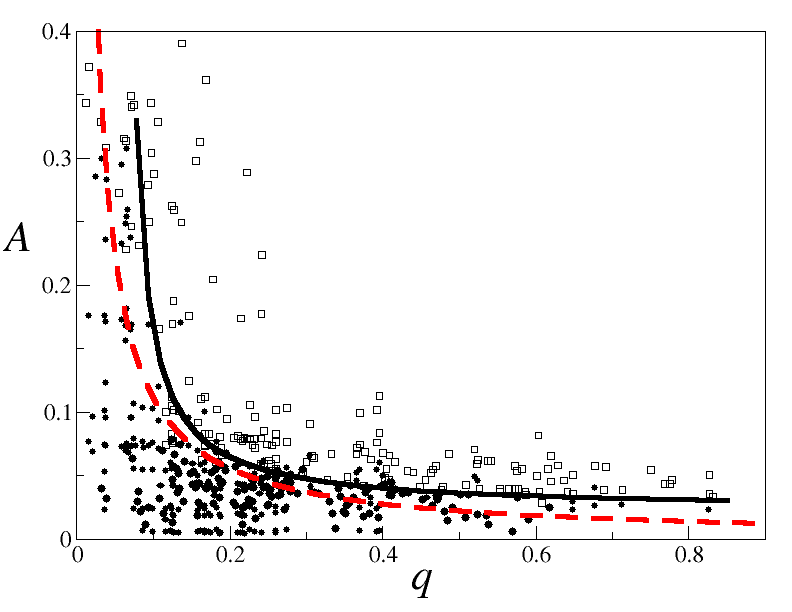
\includegraphics[width=0.8\textwidth]{polydisperse/mono1.png}\end{center}
	\caption[Crystallizability of monodisperse aspherical particles vs. $A$ and $q$]{Crystallizability of monodisperse aspherical particles characterized in terms of two shape parameters $A$ and $q$. Filled circles indicate particles that easily crystallized, while open squares indicate particles that did not.  The solid line is a guide to the eye constructed between the two distinct regions in which particles crystallize or not.  The dashed line represents a prediction of the crystallizability limit from above, $Aq = \simeq 0.011$.}\label{mono1}
\end{figure}
It is obtained by collecting 
the crystallizability of the 487 systems built out of the 487
different particle geometries we have generated across the $A$, $q$ spectrum. 
Each point in the $A$ vs $q$ diagram represents the result of a set of simulations at different pressures.
As would be expected, crystallization is favored when both $A$ and $q$ are small -- that is, 
when the particles are nearly spherical by both measures.  
A roughly inverse relationship is clearly evident; particles with large $A$ must have very small $q$ in order to have
a hope of crystallization, and vice-versa.
But more importantly, we find the existence of a clear boundary delineating the crystallizability limit 
for every possible shape generated with our model (small deviations at the interface are
likely due to finite size effects and/or the limited length of our simulations).

This is quite remarkable because it provides a very useful way of predicting whether a particular particle shape can pack into a
crystalline structure by simply measuring the experimentally accessible $A$ and $q$. 

Notice that for smaller values of $q$ our data seem to 
indicate a sharp end of the crystal boundary. We believe this to be an artifact of our particle model.
In fact, that region is where the value of $\sigma_0$ becomes sufficiently  large ($\sigma_0>0.5\sigma$)
to break the compactness of the particles generated with our method, especially those with smaller values of $N_b$. 
Furthermore, as small values of $q$ indicate a large orientational symmetry, we expect this
region to be heavily populated by specific  geometric arrangements (as discussed below), whose packing properties, at large values of $A$,
will be extremely sensitive of the particular value of $N_b$. 

As our model is intended to describe randomly shaped particles, 
our diagram does not include the results for particles designed with very specific shapes such as rods,
plates or regular polyhedral geometries that are known to crystallize. 
These particular cases would generate sharp peaks around specific values of $q$. 
Furthermore, is not clear that our two order parameters, which have after all been selected to describe asphericity, 
would be the most appropriate to study deviations from an arbitrary nonspherical designed shape. 
We therefore limited our study to $N_b >3$, to explicitly avoid trivial cases such as rod-like ($N_b=2$) and plate-like particles ($N_b=3$).

The dashed line in Figure~\ref{mono1} is the limit $Aq \lesssim 0.011$ attained in Section~\ref{sec:polydisperse}.
Although it is not a perfect division, likely due to many factors (including finite-size effects), this simple prediction provides a reasonable dividing line which would predict the crystallization or non-crystallization of 387 of the 487 systems tested, or almost 80\%.
Given the uncertainties discussed above associated with the data points,  we believe this is a remarkably good rate of success.

\section{The character of crystals of aspherical particles}

Two obvious questions present themselves in the face of these data.
The first is: what is the nature of the crystals formed when particles do crystallize; 
does the system present translational but not orientational order, as expected for $A\simeq 0$, or
does the rotational motion of the particles become restricted for large values of $A$?
The second is: what sets the boundary between the two phases;
do the particles that fail to crystallize do so because they become kinetically trapped or because of the 
lack of a stable crystal phase?
\begin{figure}
	\begin{center}\subfloat[]{
		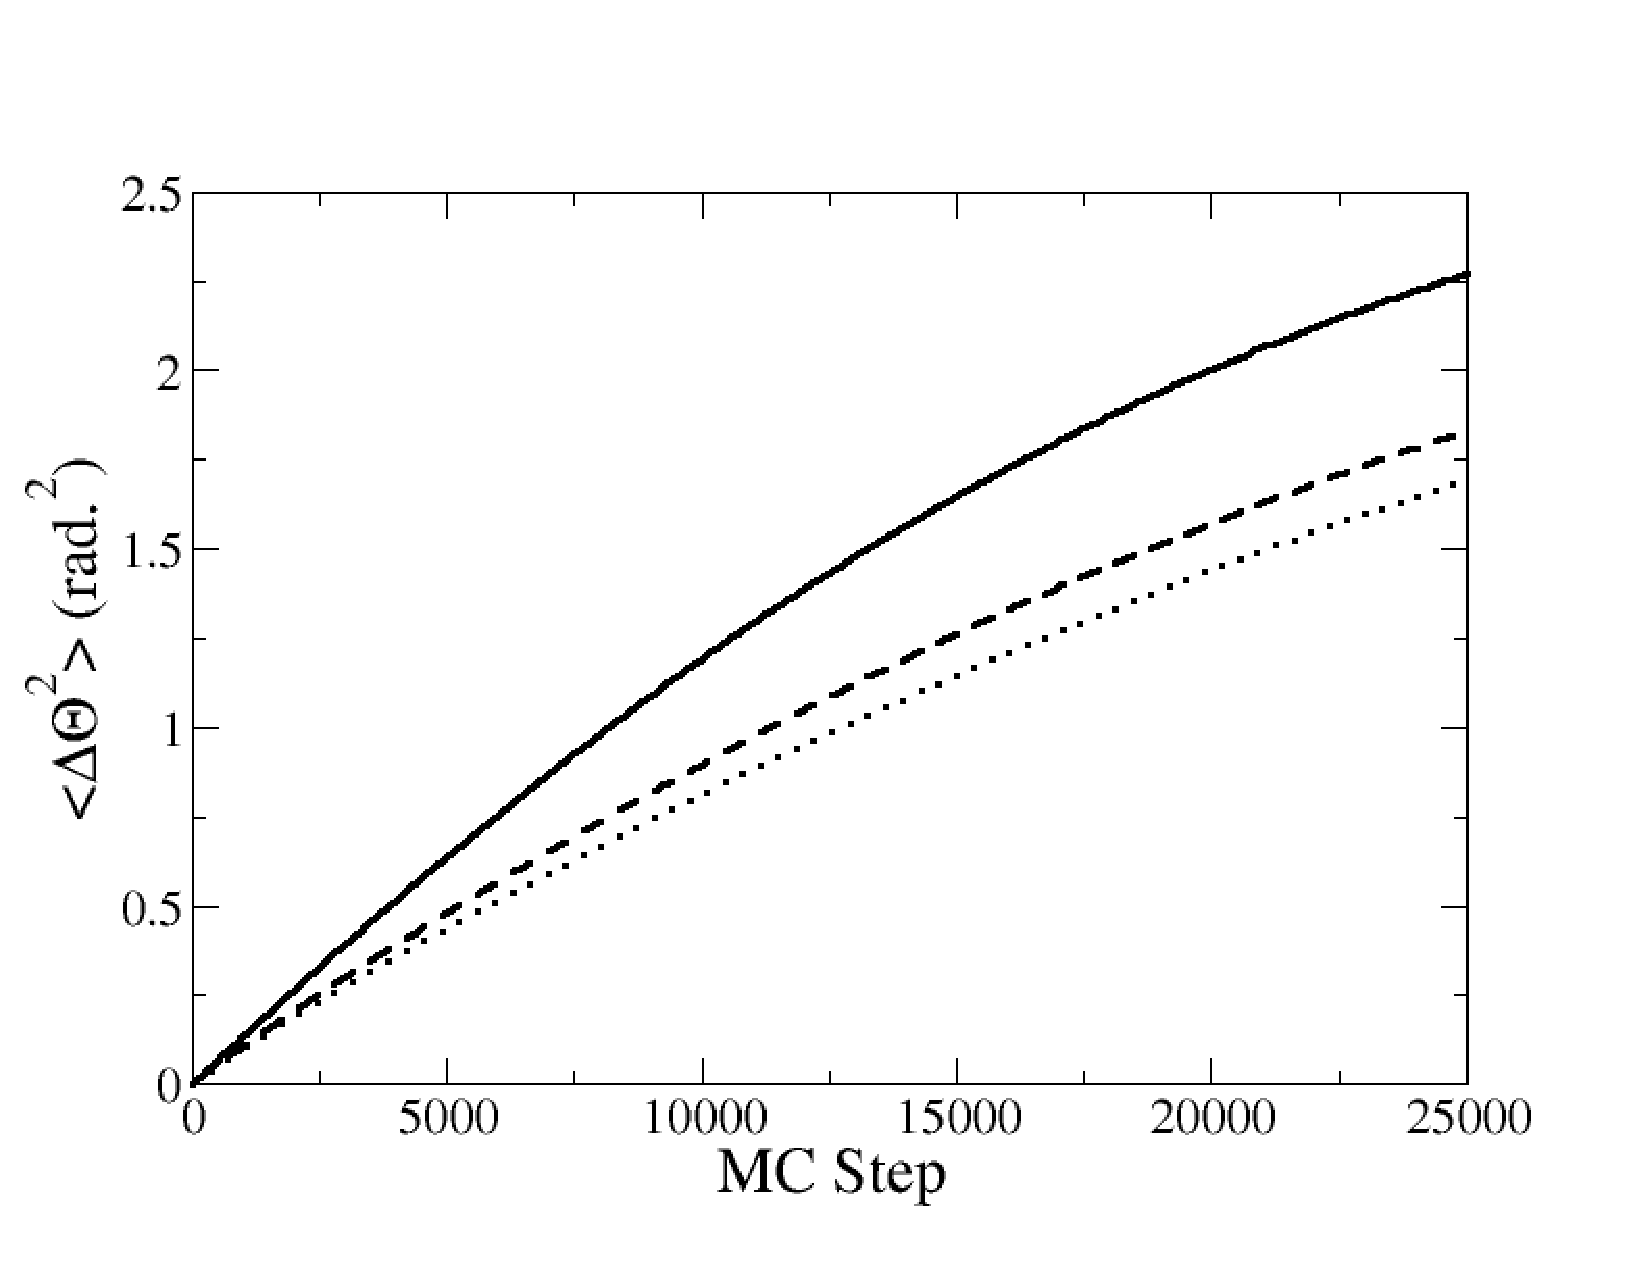
\includegraphics[width=0.6\textwidth]{disorder/rot.pdf}
		\label{rot}
	}

	\subfloat[]{
		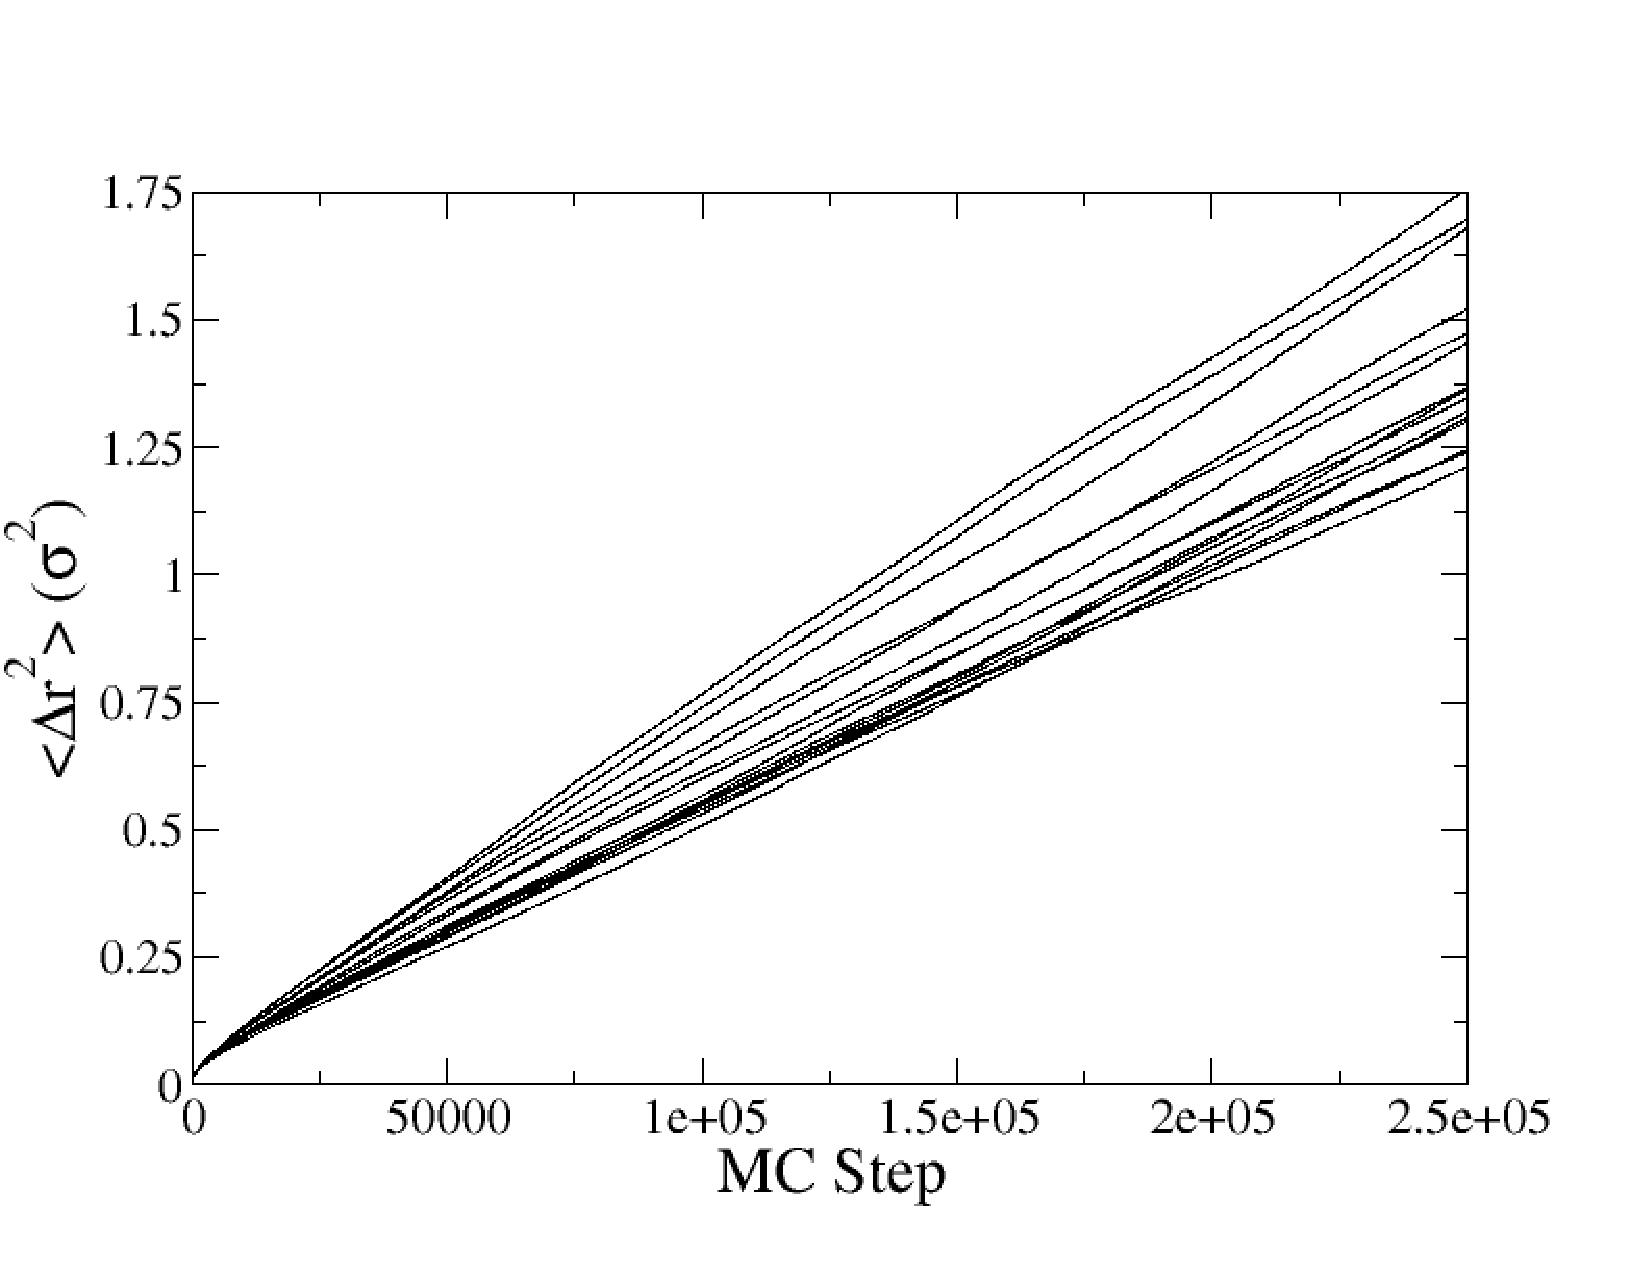
\includegraphics[width=0.6\textwidth]{disorder/trans.pdf}
		\label{trans}
	}\end{center}
	\caption[Rotational and translational diffusion for aspherical particles]{\subref{rot} Rotational mean square displacement for a subset of the particles considered. The solid line is a 
	reference for nearly spherical particles. The dashed line is the result for  those particles that  
	 crystallized and the dotted line shows $\left<\Delta\theta^2\right>$ for those that did not.
  The data were averaged over 20 realizations in each region under the same pressure $P^*=20$.
\subref{trans} Translational mean square displacement for  20 different particle shapes that failed to crystallize.}\label{diff}
\end{figure}

To address the first question, we measured the rotational diffusion, $\left<\Delta\theta^2\right>$, for 20 systems 
that crystallize, all at a reduced pressure $P^* = 20$ and near the phase boundary.  As a reference 
we also plotted  $\left<\Delta\theta^2\right>$ for nearly spherical particles, obtained by setting $\sigma_0 = 10^{-4}\sigma$, 
where we know particles are free to rotate at their lattice sites.

As can be seen in Figure~\ref{rot}, we find no evidence that particles in the crystalline phase become 
orientationally arrested or manifest an orientationally anomalous behavior. The only effect is that of decreasing their diffusion constant, 
but this is expected from simple geometrical considerations. It is obvious that at very large densities, 
regardless of the specific phase a system selects, particles' orientations will manifest a glassy behavior or eventually freeze.~\cite{schweitzer} 

It is therefore of interest to also look at the dynamical
properties of those particles in systems which do not crystallize and are located 
just across the phase boundary from the ones that do crystallize. 
These results, obtained at the same reduced pressure $P^*=20$, are also shown in Figure~\ref{rot}. 
We find no signature of anomalous dynamics, neither in the rotational (Figure~\ref{rot}), nor in the translational 
(Figure~\ref{trans}) degrees of freedom; that is, such systems behave as regular fluids.

This rotational plasticity in crystals of these aspherical particles provides and explanation for why the results of the polydisperse systems studied in Section~\ref{sec:polydisperse} applied to the monodisperse systems studied in Sections~\ref{sec:disorderpress} and~\ref{sec:disorderyesno}.
The practical effect of this fact is  
that any two identical neighboring particles will typically be misoriented and face each other with random regions of their respective surfaces. 
As a consequence, their mutual interaction becomes  hardly distinguishable, on average, from that of two particles with different shape, thus explaining why monodisperse and polydisperse 
systems may indeed present analogous equilibrium properties. 

Note, however, the deviations from the predicted pattern in Figure~\ref{mono2}
 at  the extreme ends of $Aq$,  corresponding to particle shapes that have values of $q$ significantly 
different from the average $q$ of the distribution. The deviation at large $q$ is expected as the analogous behavior is observed for polydisperse systems;
as particles become more anisotropic their rotational degrees of freedom are reduced until they perfectly align in the $q\rightarrow 1$ (rod) limit, making 
the averaged random-shape argument described above inappropriate.

A  bit more surprising is the deviation for very small values of $q$, for which we find that the polydisperse system with $N_b=12$ nicely follows the master curve.
To rationalize this behavior one has to realize that for small values of $N_b$, when $q\rightarrow 0$, particles tend to acquire rather symmetric and specific geometries, such as platonic solids, which 
also require orientational ordering  to tile the space as soon as $A$ becomes sufficiently large. These specific particle shapes dominate the shape space for $q\sim 0$ and small values of $N_b$,
and lead to deviations from the inverse power law behavior.  

This result is by no means conclusive, as a thorough investigation of this last point would require larger system sizes 
and an event-driven dynamics of the components.  Our results seem to suggest that what sets the location of 
the phase boundary is not a sudden slowdown of the dynamics of the system, but more likely
 an increase of the Gibbs free energy difference between the crystalline  and the fluid phase, analogous to
that found for polydisperse spherical particles~\cite{frenkel2}. 
It would be interesting to investigate the equilibrium properties and the stability of 
candidate crystalline structures for different values of $A$ and $q$ to investigate whether our boundary line 
coincides with the onset of crystal instability, but for the reasons given above, we have not attempted to do so.
